\section{Data-driven Reduced-order Modeling}\label{sec:dataDrivenModeling}

In recent years, the term ``data-driven'' has become a veritable buzzword in many fields, including medicine, finance, agriculture, logistics, and engineering. Although designs and applications vary widely, data-driven methods generally follow the same core process:

\begin{enumerate}
    \item Gather real-world information about an extremely complex system which humans cannot parse efficiently.
    \item Feed this data into an algorithm which learns to map the input data to meaningful output targets which are easily parsed by humans.
    \item Use the model to make useful predictions on new, unseen data.
\end{enumerate}

Such models are crucial in situations where a process cannot be readily queried (patients cannot be forced to enroll in a clinical trial), or the process must be queried many times (personalized ads must be tailored for millions of search engine users). The design of rocket combustors exhibits both challenges in some of their most extreme forms. Experimental test articles are costly to manufacture and hazardous to test. Further, rocket engines must be tested repeatedly to certify performance and safety standards. Developing reliable, approximate models that can replace (some of) these experiments has the potential to accelerate rocket design programs and lower their cost significantly. This idea reflects a broader effort in computational physics which seeks to address so-called \textit{many-query problems}, in which a model must be evaluated many times to ensure the targeted outcome is confidently estimated. Such problems include optimization, uncertainty quantification, rare event prediction, and control, all crucial element in developing robust solutions to modern engineering problems. However, the cost of existing lower-fidelity physics models, such as single-phase models for turbulent spray combustion, is often still prohibitively high and precludes their use in many-query operations. This motivates the use of data-driven modeling to discover new, inexpensive models which can be queried at a fraction of the cost of standard models.

Data-driven modeling is not new. Linear regression has been used extensively for over two centuries, and many statistical models still used regularly in modern times (e.g., k-means clustering, principal component analysis) were formulated over 50 years ago~\cite{dataScience}. What has changed in recent years is the exponential growth in computing power, data storage, and data collection mechanisms available to data scientists, as well as increased access to publicly available datasets made possible by the Internet. This same phenomenon has occurred in engineering research, where huge experimental and DNS datasets can be easily exchanged, standardized data formats allow for quick data ingestion, and open-source and hardware/software interoperability programs permit rapid verification and validation of numerical experiments. This wealth of high-fidelity data has enabled a rapid expansion of research in methods which learn low-cost models of complex physical processes, often referred to as \textit{reduced-order models}, (ROMs) where ``order'' refers to the dimensionality of the problem.

The phrase reduced-order model (sometimes \textit{reduced models} or \textit{model order reduction}) has taken on two distinct meanings in the fluid mechanics and combustion literature. The first type of ROM refers to models which are derived by simplifying complex physics with physically-meaningful (but lower-cost) approximations, or by fitting compact analytical equations to empirically-observed patterns. Examples of the former (which are not necessarily data-driven) include axisymmetric models of three-dimensional systems, or flame transfer function models of gas turbines~\cite{Schuller2002}. The latter includes polynomial models of gas thermodynamic and transport properties~\cite{McBride1993}, or Arrhenius rates for chemical reactions. For this type of ROM, the result of order reduction (relative to, perhaps, DNS or molecular reaction models) is a secondary consequence of approximating physical processes. In this sense, this type of model is henceforth referred to instead as a \textit{reduced-physics model}. While these play a critical role in developing computationally-tractable models, and play a secondary role in the results presented in this thesis, they are not the focus of this work.

The second type of ROM, central to this work, refers to models which learn a mapping from a low-dimensional representation of the system state to the full-dimensional state, and provide a means of evolving this low-dimensional representation in time. Figure~\ref{fig:mappingVis} illustrates a simple example of this process, showing the evolution of a reduced-order state in two dimensions and the corresponding full-order state in three dimensions. At their core, these methods attempt to recreate the behavior of the full-dimensional system, not that of a physically-simplified surrogate. The low-dimensional state is often a mathematical construct without particular physical significance. In this case, order reduction is a direct consequence of the mapping from low- to high-dimensional states. As such, \textit{reduced-order model} seems more appropriately applied to these models, and use the acronym ROM to refer to them exclusively.

\begin{figure}
	\begin{minipage}{0.49\linewidth}
		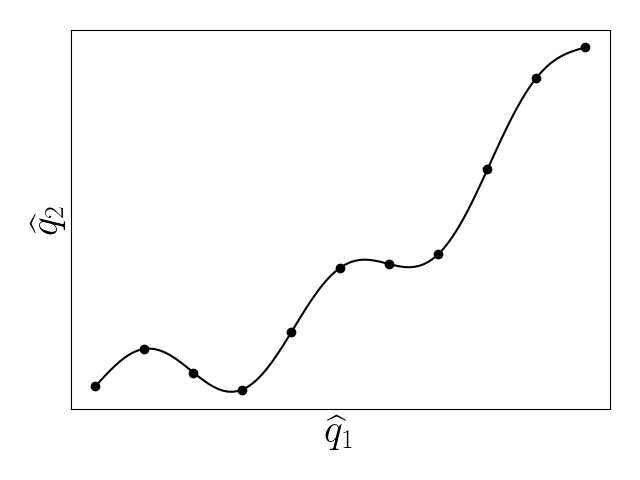
\includegraphics[width=0.99\linewidth]{Chapters/Overview/Images/mapExample_2d.png}
	\end{minipage}
	\begin{minipage}{0.49\linewidth}
		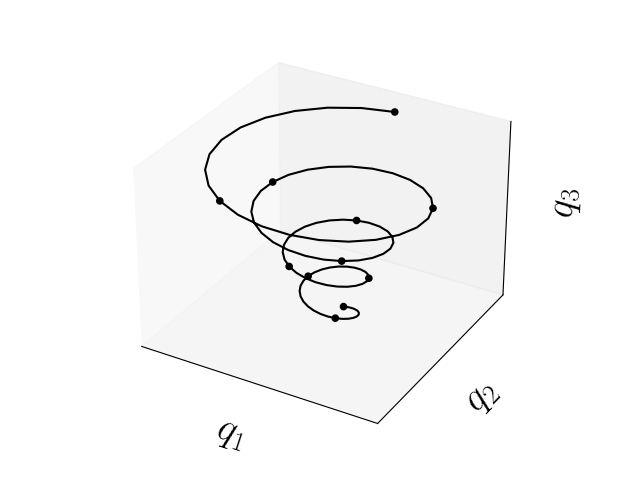
\includegraphics[width=0.99\linewidth,trim={3em 1.5em 3em 4em},clip]{Chapters/Overview/Images/mapExample_3d.png}
	\end{minipage}
	\caption{\label{fig:mappingVis}Illustration of state representation and time evolution in reduced-order space (left) and corresponding full-order state (right).}
\end{figure}

All ROMs begin by defining the mapping from a low-dimensional reduced space to the high-dimensional physical space. This mapping may be categorized broadly as linear or non-linear. Linear methods reconstruct the high-dimensional state from a linear combination of a small number of basis vectors. The scalar coefficients of this linear combination represent the low-dimensional state. Prominent methods for computing the basis vectors from data including proper orthogonal decomposition~\cite{berkoozPOD}, balanced truncation~\cite{Gugercin2004}, and the reduced-basis method (RBM)~\cite{reducedBasisBook}. Non-linear methods, on the other hand, formulate the mapping as an arbitrarily non-linear function of the low-dimensional state. Examples include autoencoders~\cite{Kramer1991}, kernel principal component analysis~\cite{kernelPCA}, and generative topographic mappings~\cite{Bishop1997}. In practice, linear and non-linear mapping methods differ in their ease of calculation and expressiveness. Linear methods benefit from closed-form solutions, and the mapping from the reduced to full-order space amounts to simple linear algebra operations. However, the linear representation often results in high approximation error when applied to very non-linear solution manifolds. For example, similar to the Gibbs phenomenon of Fourier series, linear representations of sharp gradients exhibit ``ringing'' artifacts. Non-linear methods, on the other hand, may estimate such non-linearities much more accurately, though they rarely guarantee any measure of optimality and may require costly training procedures.

After the mapping has been computed, a method of evolving the low-dimensional state in time must be selected. The Koopman operator~\cite{Budisic2012}, which can be approximated by dynamic mode decomposition~\cite{Schmid2010}, is a linear operator which simply advances the state forward in time. Operator inference~\cite{Peherstorfer2016}, alternatively, learns a quadratic form of the reduced-order state time evolution via a least-squares minimization problem. A host of neural network approaches also propose to model the dynamics of the reduced state using, for example, recurrent neural networks~\cite{Gonzalez2018}, temporal convolutional networks~\cite{Xu2020}, and adversarial networks~\cite{QuilodranCasas2021}. Finally, of particular interest to this work, is the \textit{projection-based} reduced-order model.

\subsection{Projection-based Reduced-order Models}

Unlike the methods described above, projection-based ROMs (PROMs) do not discard the original governing equations which generated the high-fidelity data. Instead, they project the system onto a low-dimensional space and evaluate the resulting reduced set of equations as you might the original high-dimensional ODE. In theory, the solution to this low-dimensional system is far less expensive than that of the full-order system. The two dominant projection methods are Galerkin projection and least-squares Petrov--Galerkin (LSPG) projection. These methods will be described in greater detail in Chapter~\ref{chap:ProjROMs}, but a brief overview is provided here to highlight existing shortcomings in the state-of-the-art.

Galerkin PROMs have a rich history in the study of coherent structures in turbulence, dating back to work in turbulent boundary layers by Aubry \textit{et al.}~\cite{Aubry1988} and progressing to more complex geometries through the 1990's (e.g.,~\cite{Deane1991,Deane1994,Cazemier1998,BuiThanh2007}). However, as Galerkin PROMs were applied to more complex fluid flow systems, they were discovered to suffer from a variety of stability and accuracy issues~\cite{Rempfer2000}. Despite careful modifications targeted at PROMs for compressible flows~\cite{rowleyGpod,Kalashnikova2011}, these stability issues arguably stem from the core fact that Galerkin projection is the $\ell^2$-optimal projection of the time-continuous governing ODE, while in practice the PROM is solved in the time-discrete O$\Delta$E setting~\cite{Grimberg2020}.

In the early 2010's, LSPG projection~\cite{Carlberg2010,Carlberg2013} was proposed as a discrete-optimal alternative to Galerkin projection. It has since been well-documented to generate far more stable and accurate PROMs compared to Galerkin projection for canonical 2D and 3D fluid flow problems~\cite{Carlberg2017}. Although broader adoption of LSPG PROMs has been slow, it has performed exceptionally well for several of perhaps the largest and most challenging aerodynamics problems to date~\cite{Grimberg2021}.

In the late 2010's, early work began in applying Galerkin and LSPG PROMs to reacting flow problems. Preliminary results indicated that these PROMs struggled with the stiff chemical kinetics and steep gradients which are characteristic of combusting flows~\cite{Huang2018a,Huang2018b}. While \textit{ad hoc} solutions of temperature limiters~\cite{Huang2019} and chemical species limiters~\cite{Huang2020} alleviated these difficulties somewhat, the general robustness of these PROMs remained poor.  It was not until very recently that the model-form preserving least-squares with variable transformation (MP-LSVT)~\cite{Huang2022} was proposed as an alternative to LSPG which exhibits greatly improved performance for PROMs of reacting flows.

Several key limitations remain to be solved for PROMs of general non-linear problems, namely computational efficiency and predictivity. As will be discussed in Chapter~\ref{chap:HPROMS}, PROMs of non-linear systems require a hyper-reduction method to limit the cost of evaluating non-linear terms in the governing ODE. Very little research has been conducted to compare the performance of various hyper-reduction approaches, beyond studies of small one-dimensional systems~\cite{Peherstorfer2020}. Further, prior work on PROMs of large-scale systems typically do not explore performance beyond training data sets, i.e. predictive performance. Recent work implies that online adaptation of the PROM basis and hyper-reduction sampling scheme provide vastly improved predictive performance~\cite{Peherstorfer2022,WayneIsaacTanUy2022}, though these methods have yet to be tested for high-dimension, multi-scale systems.
